\documentclass{beamer}
\usepackage{polski}
\usepackage[utf8]{inputenc}
\usepackage{graphics}
\usepackage{minted}
\usepackage{fvextra}
\usepackage{caption}
\usepackage{epigraph}
\usepackage{array}
\newcolumntype{L}[1]{>{\raggedright\let\newline\\\arraybackslash\hspace{0pt}}m{#1}}
\newcolumntype{C}[1]{>{\centering\let\newline\\\arraybackslash\hspace{0pt}}m{#1}}
\newcolumntype{R}[1]{>{\raggedleft\let\newline\\\arraybackslash\hspace{0pt}}m{#1}}
\definecolor{NiceGreen}{RGB}{40,200,0}
\definecolor{CoolDarkGray}{RGB}{50,50,50}


\title{\texttt{Projekt aplikacji do ekstremalnego uczenia maszynowego do klasyfikacji big data}}
\author{Ahmed Abdelkarim, Aleksandra Hernik}

\begin{document}
\setbeamercolor{background canvas}{bg=CoolDarkGray}
\setbeamercolor{title}{fg=NiceGreen}
\setbeamercolor{frametitle}{fg=NiceGreen}
\setbeamercolor{structure}{fg=white}
\setbeamertemplate{section in toc}{%
    \textcolor{NiceGreen}{\inserttocsectionnumber)}   \inserttocsection \par}

\addtobeamertemplate{navigation symbols}{}{%
    \usebeamerfont{footline}%
    \usebeamercolor[fg]{footline}%
    \hspace{1em}%
    \insertframenumber/\inserttotalframenumber
}

\setbeamercolor{normal text}{fg=white}\usebeamercolor*{normal text}
\begin{frame}
  \maketitle
\end{frame}

\begin{frame}{Plan}
  \tableofcontents[currentsection]
\end{frame}

\section{Przypomnienie}
\begin{frame}{Przypomnienie}
\begin{figure}[H]
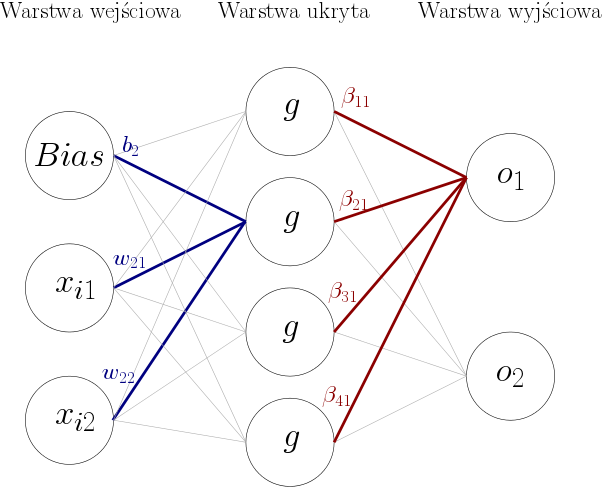
\includegraphics[scale=0.5]{schemat_sieci.png}
\caption{Sieć ELM}
\end{figure}
\end{frame}
\begin{frame}{Przypomnienie}
\begin{itemize}
\item Problem klasyfikacji
\item Wagi wejściowe losowane
\item Uczenie polega na wyznaczeniu wag wyjściowych
\item Celem ELM jest szybkość
\end{itemize}
\end{frame}
\section{Wyniki}
\begin{frame}{Wyniki meczów w grze Dota2}
\begin{itemize}
\item 50 000 próbek
\item 10 kolumn
\item 2 możliwe klasy
\end{itemize}
\begin{table}[H]
\caption{Przykładowe dane}
\begin{tabular}{|c|c|c|c|c|c|c|c|c|c|}
\hline
2375 & 1982 & 4 & 3 & 63 & 1 & 22 & 0 & 1 & 155 \\
2582 & 0 & 1846 & 63 & 0 & 221 & 22 & 0 & 2 & 154 \\
2716 & 256 & 1972 & 63 & 48 & 190 & 22 & 0 & 0 & 132 \\
3085 & 4 & 1924 & 51 & 3 & 40 & 22 & 0 & 0 & 191 \\
1887 & 2047 & 0 & 0 & 63 & 58 & 22 & 0 & 0 & 156 \\
\hline
\end{tabular}
\end{table}

\end{frame}

\begin{frame}{Dota2 w Pythonie}
\begin{figure}[H]
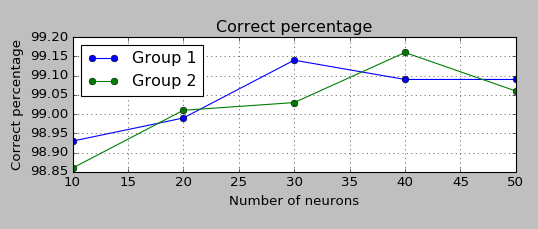
\includegraphics[width=\textwidth]{wyniki_dota2_python_percentage.png}
\caption{Jakość uczenia}
\end{figure}

\end{frame}

\begin{frame}{Dota2 w Pythonie}
\begin{figure}[H]
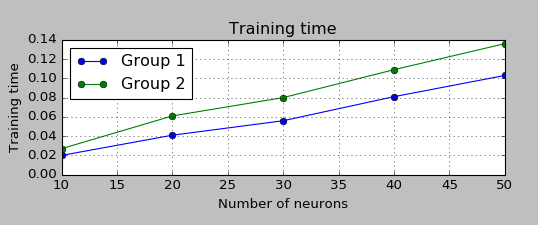
\includegraphics[width=\textwidth]{wyniki_dota2_python_training_time.png}
\caption{Czas uczenia}
\end{figure}

\end{frame}

\begin{frame}{Dota2 w Pythonie}
\begin{figure}[H]
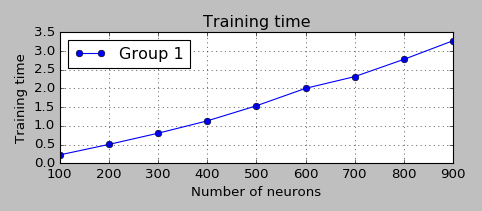
\includegraphics[width=\textwidth]{wyniki_dota2_python_training_time_2.png}
\caption{Czas uczenia - więcej neuronów}
\end{figure}

\end{frame}


\begin{frame}{Dota2 w Matlabie}
\begin{figure}[H]
\centering
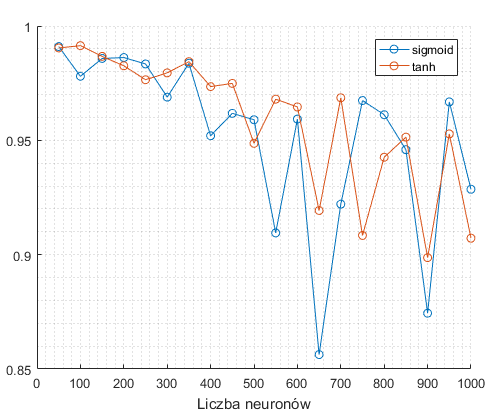
\includegraphics[width=0.85\textwidth]{dota_liczba_neuronow.png}
\caption{Jakość uczenia}
\end{figure}
\end{frame}

\begin{frame}{Dota2 w Matlabie}
\begin{figure}[H]
\centering
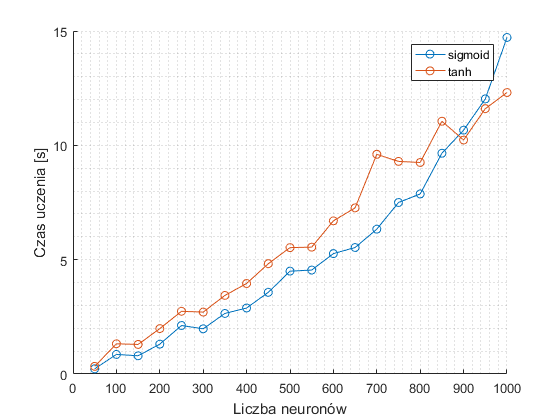
\includegraphics[width=0.85\textwidth]{dota_wydajnosc.png}
\caption{Czas uczenia}
\end{figure}
\end{frame}

\begin{frame}{Dominujący gatunek drzew w lesie}
\begin{itemize}
\item 15 120 próbek
\item 54 kolumny, w tym 44 binarne
\item 7 możliwych klas
\end{itemize}
\begin{table}[H]
\caption{Przykładowe dane z pominięciem 44 binarnych kolumn}
\begin{tabular}{|c|c|c|c|c|c|c|c|c|c|}
\hline
2596 & 51 & 3 & 258 & 0 & 510 & 221 & 232 & 148 & 6279 \\
2590 & 56 & 2 & 212 & -6 & 390 & 220 & 235 & 151 & 6225 \\
2804 & 139 & 9 & 268 & 65 & 3180 & 234 & 238 & 135 & 6121 \\
2785 & 155 & 18 & 242 & 118 & 3090 & 238 & 238 & 122 & 6211 \\
2595 & 45 & 2 & 153 & -1 & 391 & 220 & 234 & 150 & 6172 \\
\hline
\end{tabular}
\end{table}
\end{frame}

\begin{frame}{Lasy w Pythonie}
\begin{figure}[H]
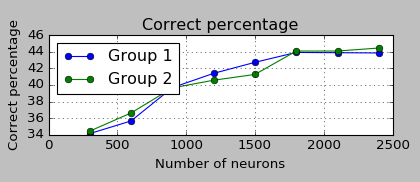
\includegraphics[width=\textwidth]{wyniki_forest_python_percentage.png}
\caption{Jakość uczenia}
\end{figure}
\end{frame}

\begin{frame}{Lasy w Pythonie}
\begin{figure}[H]
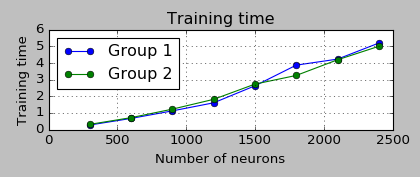
\includegraphics[width=\textwidth]{wyniki_forest_python_training_time.png}
\caption{Czas uczenia}
\end{figure}
\end{frame}

\begin{frame}{Lasy w Matlabie}
\begin{figure}[H]
\centering
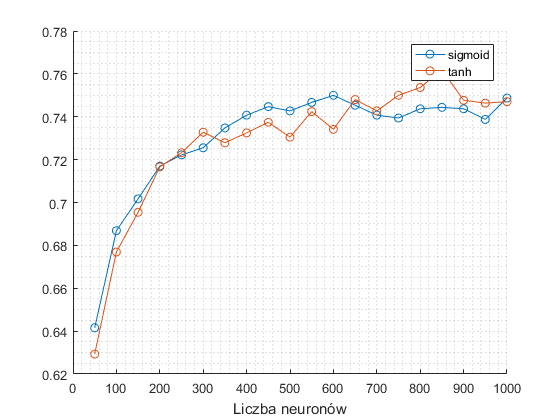
\includegraphics[width=0.85\textwidth]{forest_liczba_neuronow.png}
\caption{Jakość uczenia}
\end{figure}
\end{frame}

\begin{frame}{Lasy w Matlabie}
\begin{figure}[H]
\centering
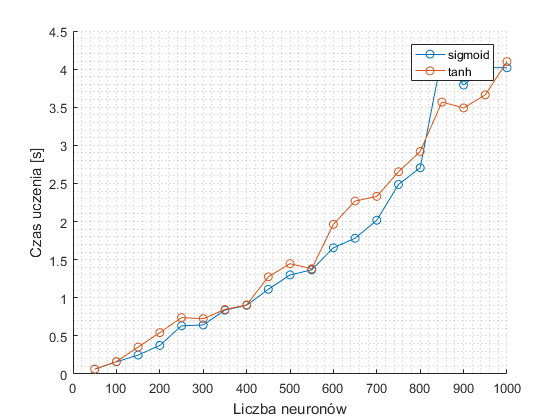
\includegraphics[width=0.85\textwidth]{forest_wydajnosc.png}
\caption{Czas uczenia}
\end{figure}
\end{frame}

\section{Wnioski}
\begin{frame}{Różnice w implementacjach}
\begin{itemize}
\item Normalizacja
\item Sposób losowania wag wejściowych
\item Potencjalna rozbieżność biblioteki z teorią
\end{itemize}
\end{frame}

\begin{frame}{Wnioski}
\begin{itemize}
\item ELM rzeczywiście działają bardzo szybko
\item ELM radzą sobie z nietypowymi danymi
\item Normalizacja jest bardzo istotna
\item Drobne różnice w implementacji powodują zupełnie inne wyniki
\item Zależność czasu uczenia od liczby neuronów jest nieliniowa
\item Zwiększanie liczby neuronów poprawia rezultaty tylko do pewnego momentu
\end{itemize}

\end{frame}

\begin{frame}
\begin{center}
\huge{Dziękujemy za uwagę}
\end{center}

\end{frame}

\end{document}
\endinput